		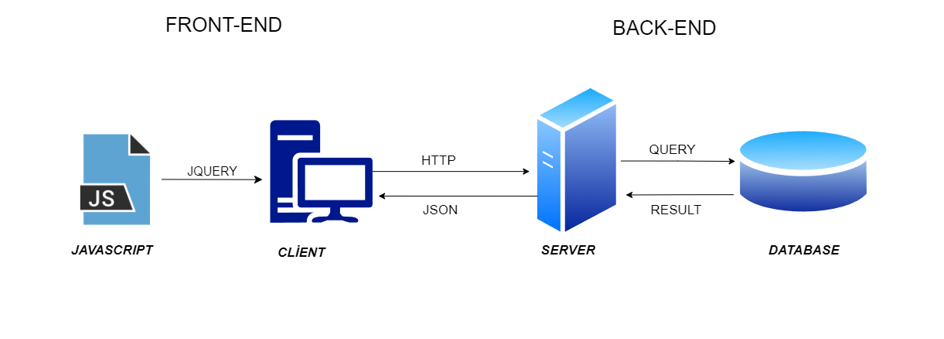
\includegraphics[width=\textwidth,keepaspectratio]{isleyis.png}



Projenin 4 katmanlı bir yapıda olduğunu belirtmiştim. Katmanlarda sırasıyla bahsedecek
olursam öncelikle Javascript katmanından başlamak isterim. Javascript katmanında jquery ile
ajax ve isteği oluşturup bir olayın tetiklenmesini sağlıyorum. Bu olay tetiklemesi
sonucunda client bir http isteği gönderiyor. Bu http isteği server katmanında tetiklenen olaya göre
içerde bir sorguyu çalıştırıyor. Bu sorgu veri tabanına bağlanarak veri tabanında gerekli işlmeleri 
gerçekleşririp bir result dönüyor. Server katmanına gelen bu result json formatta client katmanına geliyor.
Bu projenin 4 katmanlı olmasını sağlayan durum web sayfasının server tarafından hazır halde gelmeyip javascript 
katmnaında dinamik olarak hazırlanıyor olmasından kaynaklıdır.


Server tarafında, projenin iş mantığını ve veri tabanı etkileşimini yönetmek amacıyla .NET CORE üzerinde yazıp ASP.NET MVC modelini kullancağım. MVC mimarisi, uygulamayı modülerleştirir ve işlevselliği katmanlara bölerek daha yönetilebilir bir yapı oluşturur. Model katmanı, veri tabanına erişim ve veri tabanı ilişkileri gibi veri işleme süreçlerini içerir. View katmanı, kullanıcının etkileşimde bulunduğu arayüzü temsil ederken, Controller katmanı, kullanıcı komutlarını alarak bu komutları işleyen ara bir katman olarak görev yapar. Bu sayede, sistemin hem veri tabanı yönetimi hem de iş mantığı daha düzenli ve modüler bir yapı kazanmasını sağlayacaktır.
Asp.Net MVC modeli hakkında araştırmalarda kullanılmıştır.\cite{sozerihayatimda}
\vspace{1\baselineskip} %


MVC mimarisini kullanırken aynı zamanda SOLID prensiblerine uygun sekilde
kod yazmayı planlıyorum. SOLID prensiblerinden bahsedecek olursam beş temel ilkeye 
dayanıyor. SOLID prensipleri, yazılım geliştirme sürecinde kodun okunabilirliğini, bakımını,
esnekliğini ve yeniden kullanılabilirliğini artırmak için önemlidir. Bu prensiplere uygun kodlar,
daha az hata içerir, daha kolay anlaşılabilir ve daha sürdürülebilirdir. \newline 
Bu ilkeler ile ilgili araştırmamı ... adresinden yapmış bulunmaktayım.\cite{turan2018solid}\newline 
Aynı zamanda [\url{https://chat.openai.com/c/d70b0aba-f98f-4fad-a808-5ec4815176d4} ile de yararlandım.]
\vspace{1\baselineskip} %



Frontend tarafında ise JavaScript kullanarak sayfaları dinamikleştirme işlevselliği eklemeyi planlıyorum. HTML ve CSS, kullanıcı arayüzünü tasarlamak ve düzenlemek için kullanılacaktır. Bu sayede, kullanıcılar kitapları daha etkileşimli bir şekilde listeleyebilecek, arayabilecek ve filtreleyebileceklerdir.

Bu proje, modern teknolojilerin entegrasyonunu kullanarak uygulama geliştirme sürecindeki önemli konulara odaklanmakta ve hem veritabanı yönetimi hem de web uygulaması geliştirme konularında öğrenmeye yönelik bir deneyim sunmaktadır. Bu seçilen teknolojiler, projenin amacına uygun olarak sistemin etkili bir şekilde işleyişini destekleyeceği fikrindeyim.


	\begin{landscape}
\begin{figure}[h]
	\caption{GANTT CHART}
	\centering
	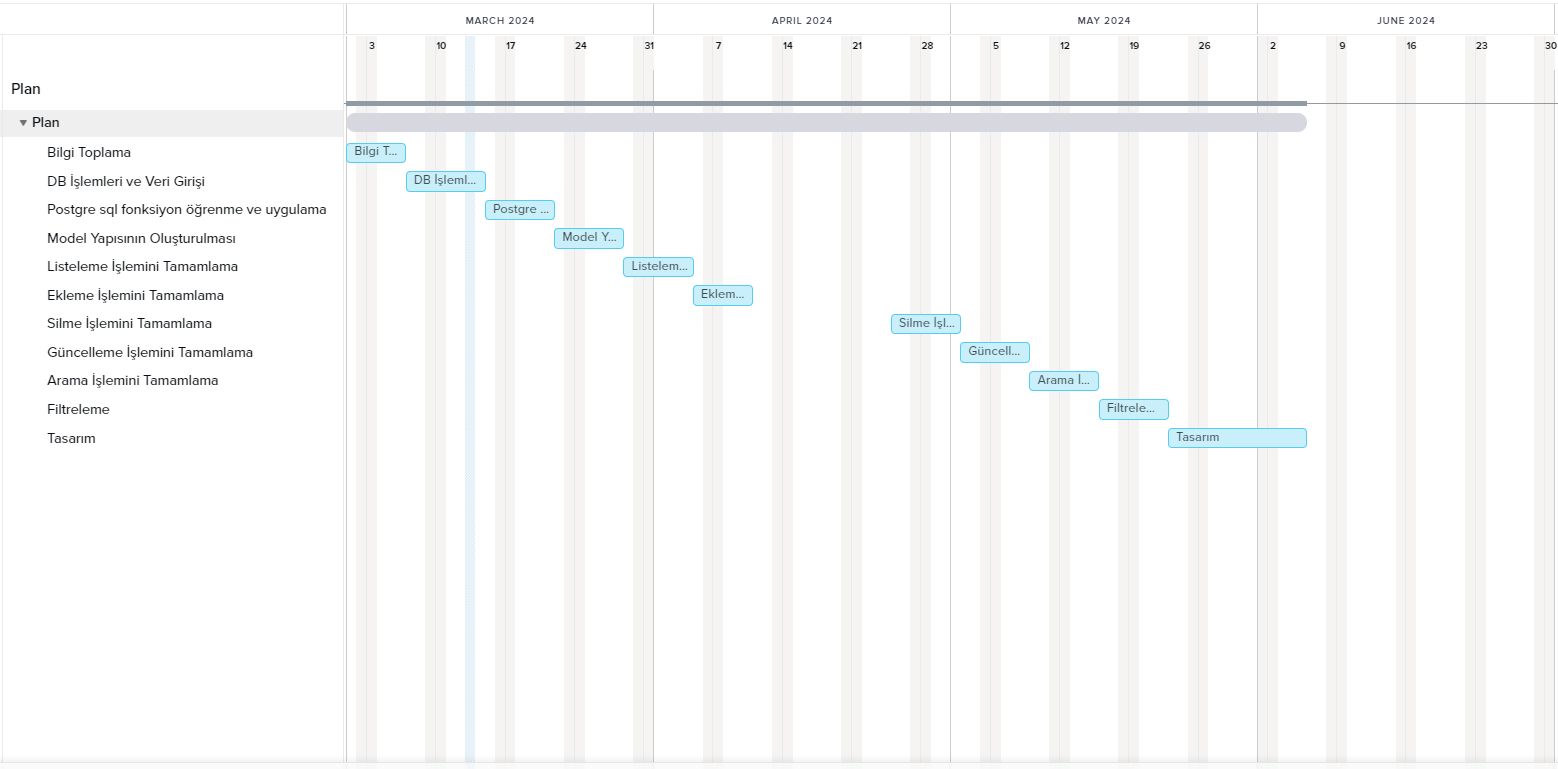
\includegraphics[width=\paperwidth,height=\paperheight,keepaspectratio]{plan.png}
	\label{gantt}
	Şekil  \ref{gantt}'de görebileceği üzere
	iş akış planı gösterilmektedir.
\end{figure}
\end{landscape}


